\section{Challenges}

During our study, we have identified five characteristics of \glspl{adptSyst} that bring challenges to the software engineering research community.
First, information gathered is not always known with absolute confidence.
Second, reconfigurations may not be immediate, and their effects are not instantaneously measured.
Third, system behaviour may be emergent~\cite{zio2011uncertainties}, \ie it cannot be entirely known at design time.
Four, the different sub-parts of the system do not evolve at the same rate.
Five, structure and behaviour of systems have a time dimension.
The last one has been published in our vision paper regarding time awareness in \gls{mde}~\cite{DBLP:conf/models/Benelallam0MFBB17}.
In this section, we detailed them.

\subsection{Engineering uncertainty-aware software}
\label{sec:intro:challenges:duc}

\begin{figure}
	\centering
	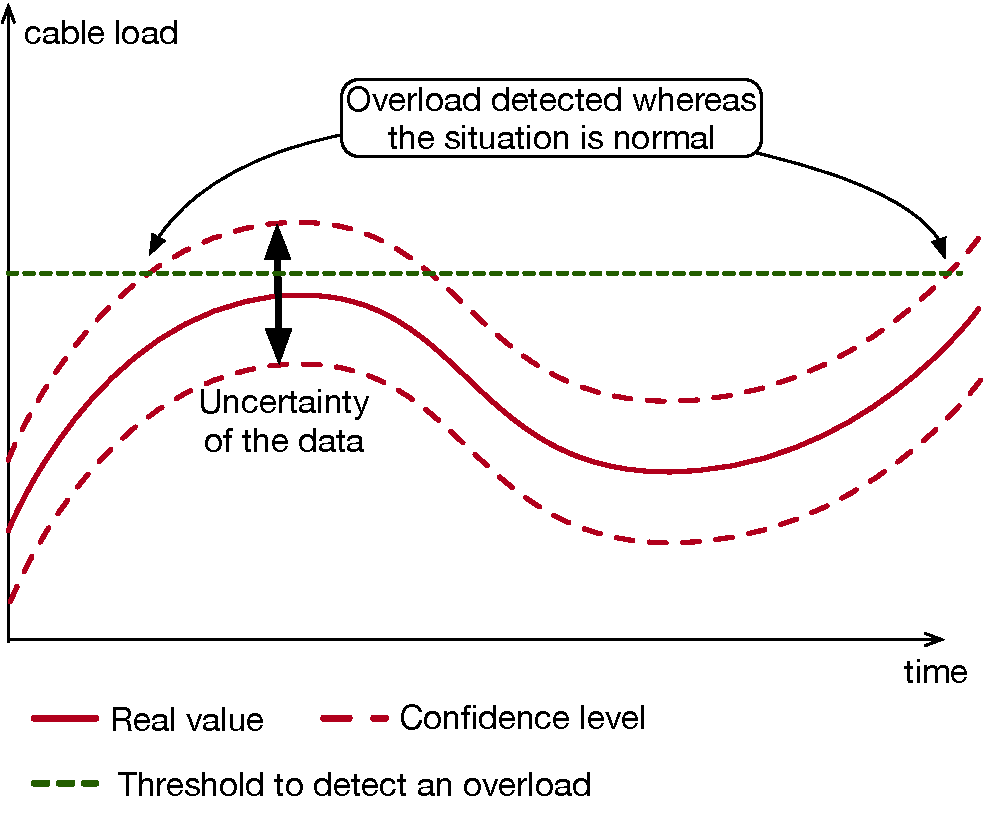
\includegraphics[width=.6\linewidth]{img/chapt-intro/challenges/duc}
	\caption{Illustration of the problem due to data uncertainty}
	\label{fig:intro:chal:duc}
\end{figure}

Most fuses are manually open and close by technicians rather than automatically modified.
Then, technicians manually report the modifications done on the grid.
Due to human mistakes, this results in errors.
The grid topology is thus uncertain.
This uncertainty is propagated to the load approximation, used to detect overloads in the grid.
Wrong reconfigurations might be triggered, which could be even worse than if no change would have been applied.

More generally, \textbf{data are, almost by definition, uncertain and developers work with estimates in most cases}~\cite{DBLP:conf/asplos/BornholtMM14, metrology2008evaluation, DBLP:journals/tkde/AggarwalY09}.
The uncertainty may be explained by how data are collected.
We can distinguish three categories: sensors, humans, and results of computations.
Sensors (software or hardware) always estimate the value and have a precision value due to the method of measurement~\cite{metrology2008evaluation, DBLP:conf/asplos/BornholtMM14}.
Humans are error-prone.
And computations can either give an approximation or be based on uncertain data.
This uncertainty is then propagated through all steps until the final result.

For a specific domain, this uncertainty may impact the understanding of the real situation as depicted in~\Cref{fig:intro:chal:duc}.
For example, the uncertainty of the \gls{cpu} clock is too low to damage the percentage load of the processor.
However, the uncertainty of the cable load in a smart grid may trigger false detection of an overload, as depicted in~\Cref{fig:intro:chal:duc}.
\textbf{If the data uncertainty can mislead the understanding of a system behaviour or state, then developers should implement an uncertainty-aware system.}
For \glspl{adptSyst}, this lack of confidence may trigger suboptimal adaptations.

Therefore, we argue that \gls{duc} impacts all the development stages of software, from the design to the execution.
Among the different stages, in this thesis we focus on the design one.
We firmly think that design techniques should provide mechanisms to help developers abstract and manipulating uncertain data.

The literature provides approaches to help engineers reason or manipulate \gls{duc}, or at least probability distributions.
For example, believe func-\linebreak{}tions~\cite{shafer1992dempster} help to reduce this uncertainty by combining several sources of data.
The probabilistic programming~\cite{DBLP:conf/icse/GordonHNR14} community provide frameworks and languages~\cite{url:InferNET18, baudin2017openturns} to propagate probabilities through computations.

However, from the best of our knowledge, no global study has been done to evaluate the impact of data uncertainty on the development of software.
The following challenge still remains an open question for the software engineering community:
\vspace{-2em}
\highlightbox{How to engineer uncertainty-aware software (design, implement, test, and validate)?}

\subsection[Reasoning over long-term actions]{Reasoning over \glspl{longTermAct}}
\label{sec:intro:challenges:longTermAct}

\begin{figure}
	\centering
	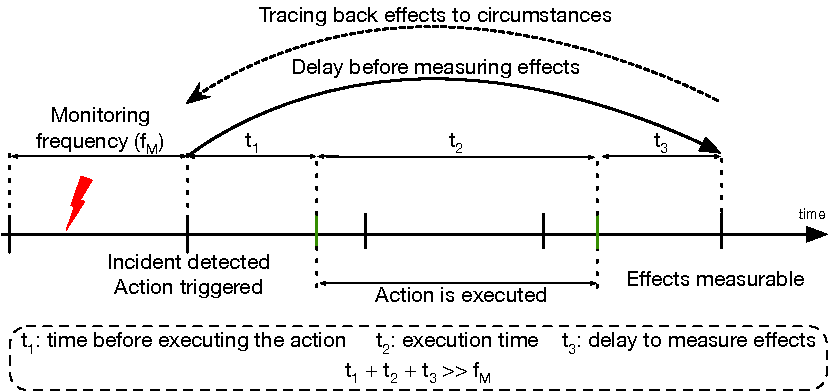
\includegraphics[width=0.9\linewidth]{img/chapt-intro/challenges/longTermAct}
	\caption{Illustration of a \gls{longTermAct}}
	\label{fig:intro:chal:longTermAct}
\end{figure}

Reconfiguring a smart grid implied to change the power flow by opening or closing fuses.
As said before, technicians need to drive physically to fuse locations to modify their states.
Besides, in the case of the Luxembourg smart grid, meters send energy measurement every 15 min, non-synchronously.
Between the time a reconfiguration of the smart grid is decided, and the time the effects are measured, a delay of at least 15 min occurs.
On the other hand, an incident should be detected in the next minutes.
If the adaptation process does not consider this difference of rates, it can cause repeated decisions.

More generally, a difference may exist between the monitoring frequency of the time for action effects to be measured.
One cause of this is what we call \glspl{longTermAct} in this document, illustrated in~\Cref{fig:intro:chal:longTermAct}.
A \gls{longTermAct} is defined as an \gls{action} that takes time to be executed  (delay to be executed and execution time) or that have long-term effects.
A second cause is an impossibility to reduce the monitoring frequency since systems must be reactive in some cases.
This difference in rates may damage the decision process.

Therefore, we argue that \textbf{decision-making processes should consider this delay if the frequency of the monitoring stage is lower than the time of action effects to be measurable}.
From the best of our knowledge, none approach allows developers implementing such tools.
One open challenge for the research community is thus:
\vspace{-2em}
\highlightbox{How to model, store, and query long-term actions with their effects?}


\subsection{Diagnosing the adaptation process}
\label{sec:intro:challenges:diagnosis}

\Gls{sg} \gls{behaviour} is affected by several factors that cannot be controlled by the grid manager.
One example is the weather conditions.
\Glspl{sg} rely on an energy production distributed over several actors.
For instance, users, who were mainly consumers before, can now produce energy by adding solar panels on the roof of their houses.
The production of such energy depends on the weather, and even on the season\footnote{The angle of the sun has an impact on the amount of energy produced by solar panels. This angle varies according to the season.}.
Despite this stochasticity of the \gls{behaviour}, engineers need to implement an adaptation process, that can lead to suboptimal grid configuration.

Faced with growingly complex and large-scale software systems (e.g. smart grid systems), we can all agree that the presence of residual defects becomes unavoidable~~\cite{DBLP:conf/icse/BarbosaLMJ17, DBLP:conf/icse/MongielloPS15, DBLP:conf/icse/HassanBB15}. 
Even with a meticulous verification or validation process, it is very likely to run into an unexpected behaviour that was not foreseen at design time. 
Alone, existing formal modelling and verification approaches may not be sufficient to anticipate these failures~\cite{DBLP:conf/icse/TaharaOH17}. 
As such, complementary techniques need to be proposed to locate the anomalous behaviour and its origin in order to handle it in a safe way.

Bencomo~\etal~\cite{DBLP:conf/iceccs/BencomoWSW12} argue that comprehensive explanation about the system behaviour contributes drastically to the quality of the diagnosis, and eases the task of troubleshooting the system behaviour. 
To enable this, as shown in~\Cref{fig:intro:chal:longTermAct}, we believe that adaptive software systems should be equipped with traceability management facilities to link the decisions made to their \textbf{(i) circumstances, that is to say, the history of the system states and the targeted requirements, and (ii) the performed actions with their impact(s) on the system}.
In particular, an \textbf{adaptive system should keep a trace of the relevant historical events}.
Additionally, it should be able to \textbf{trace the goals intended to be achieved by the system to the adaptations and the decisions that have been made, and vice versa}. 
Finally, in order to enable developers to interact with the system in a clear and understandable way, appropriate abstraction to \textbf{enable the navigation of the traces and their history should also be provided}.
In other words, the research community should answer the following global challenge:
\vspace{-2em}
\highlightbox{How to trace back adaptation decision effects to their circumstances?}

\subsection{Modelling inconsistent states of system}
Every meter sends consumption and production data every 15 min.
However, this collection is not synchronous.
That is, all meters do not send their data at the same timestamp.
The global system, which receives all data, has not thus a global vision with the same freshness for all the part of the grid.
Electricity data are volatile: a peak or a drop may happen in less than a minute due to, for instance, the starting or the finishing of a washing machine.
Reconfiguration of the grid may thus be suboptimal due to outdated information.

\textbf{Different parts of a system may evolve at different rates.}
Some systems are heterogeneous in terms of hardware and software.
This diversity results in different evolution or reaction rates.
For example, if some components are working on batteries, they will have a sleep cycle to save energy.
Contrary, if some others are running connected directly to a power source, they can react faster.

Despite this difference of rates, a global vision of a system at a precise time point may be still required.
The vision should deal with data that have different freshness.
For example, the adaptation process may require a global view of the system.
In the worst case, some data would be outdated and cannot be used.

When designing the adaptation process, engineers need thus solutions to deal with an inconsistent system state.
One solution can, for example, seamlessly estimate what should be the current value of outdated data.
One global challenge for the software engineering community is therefore:
\vspace{-2em}
\highlightbox{How to represent, query, and store inconsistent system states and behaviours?}


\subsection{Modelling temporal and interconnected data}
Power flow is impacted by consumption and production of users, and by the modifications of the topology.
Knowing the last status of the grid is as important as knowing how it evolves.
Based on the evolution, the grid operator can predict any future incidents, like overloads.
It could also compare this evolution of behaviour with a normal one to detect, for example, any malicious behaviour.

\textbf{Evolution of systems is inherently linked with a time dimension.}
Evolution and time are two related concepts.
For some systems, not only the last states are important but also how they evolve.
Then, analysis processes will investigate this evolution to know if it is a normal one or not.
They can also use this evolution to predict how systems will evolve.
Based on these predictions, they can proact on future incidents in the system.

Decisions are not made upon the last state of the system but how it evolves.
The analysis process should thus navigate both in the structure of the system and its behaviour over time.
\textbf{Engineers need efficient tooling to structure, represent, query, and store temporal and interconnected data on a large scale.}

Time in software engineering is not a new challenge.
For example, Riviera \etal \cite{DBLP:conf/models/RiveraRV08} have already identified time as a challenge for the \gls{mde} community.
Different approaches have been defined~\cite{DBLP:conf/sle/BousseCCGB15, DBLP:conf/sle/KansoT12, DBLP:conf/icse/KoegelH10, DBLP:conf/seke/0001FNMKT14}.

However, we notice that modelling, persistence, and processing of data evolution remain understudied.
Thomas Hartmann started addressing these challenging in his PhD thesis~\cite{DBLP:phd/basesearch/Hartmann16}.
The final global challenge, not fully addressed, is thus:
\vspace{-2em}
\highlightbox{How to structure, represent query, and store efficiently temporal data on a large scale?}